\documentclass[a4paper,20pt]{article} 
\usepackage{geometry}
\usepackage{wrapfig}
\geometry{
	a4paper,
	total={170mm,237mm},
	left=20mm,
	right=20mm,
	top=30mm,
}
\usepackage{titlesec}
\usepackage{tabularx}

\titlelabel{\thetitle.\quad} %точка в section

%%% Работа с русским языком
\usepackage{cmap}                           % поиск в PDF
\usepackage{mathtext} 			 	       % русские буквы в формулах
\usepackage[T2A]{fontenc}               % кодировка
\usepackage[utf8]{inputenc}              % кодировка исходного текста
\usepackage[english,russian]{babel}  % локализация и переносы

%Математика
\usepackage{amsmath,amsfonts,amssymb,amsthm,mathtools} % AMS
\usepackage{icomma} % "Умная" запятая

%% Шрифты
\usepackage{euscript}	 % Шрифт Евклид
\usepackage{mathrsfs} % Красивый матшрифт

\usepackage{mathtext} 
\usepackage{setspace}
\usepackage{tabularx}
\usepackage{longtable}
\usepackage{icomma}
\usepackage{euscript}
\usepackage{float}
\usepackage{cutwin}
\usepackage{mathrsfs}
\usepackage{adjustbox}
\usepackage{dashbox}
\usepackage[normalem]{ulem}	
\usepackage[babel=true]{microtype}
\RequirePackage[T1]{fontenc}
\usepackage{amsmath,amsfonts,amssymb,amsthm,mathrsfs,mathtools} 
\usepackage{xcolor}         
\usepackage{enumitem}     
\usepackage{xpatch}       
\usepackage{cancel}                  
\usepackage{upgreek}                 
\usepackage{lipsum}                  
\usepackage[version=4]{mhchem}       
\usepackage{multirow}                
\usepackage{stackengine}             
\usepackage{tikz}         
\usepackage{hyperref}
\hypersetup{colorlinks=true,urlcolor=blue}       
\usetikzlibrary{positioning}         
\usepackage{titletoc}                 
\usepackage{chngcntr}              
\usepackage{fancyhdr}                
\usepackage{makecell}                
\usepackage{indentfirst}             
\usepackage{tocloft}                 
\usepackage{soul}                   
\usepackage[stable]{footmisc}       
\usepackage{subfig}                  

\mathtoolsset{showonlyrefs=true}


\theoremstyle{definition}
\newtheorem*{definition}{Определение}
\newtheorem{statement}{Предложение}[section]
\newtheorem{lemma}{Лемма}[section]
\newtheorem{theorem}{Теорема}[section]
\newtheorem*{theoremn}{Теорема}
\newtheorem*{corollary}{Следствие}
\newtheorem*{example}{Пример}
\newtheorem*{note}{Замечание}
\newtheorem*{problem}{Задача}



\newcommand{\dotpr}[2]{\bra{#1}\ket{#2}}
\let\AA\relax
\let\emptyset\varnothing
\DeclareMathOperator*{\esssup}{ess sup}
\DeclareMathOperator*{\ord}{ord}
\DeclareMathOperator*{\supp}{supp}
\DeclareMathOperator*{\pr}{pr}
\DeclareMathOperator*{\Ker}{Ker}
\DeclareMathOperator*{\Vol}{Vol}
\DeclareMathOperator*{\rg}{rk}
\DeclareMathOperator*{\Ima}{Im}
\DeclareMathOperator*{\Alt}{Alt}
\DeclareMathOperator*{\Sym}{Sym}
\newcommand{\eqdef}{\stackrel{\text{\tiny{def}}}{=}}
\newcommand{\pp}{\partial}
\newcommand{\AA}{\mathcal{A}}
\newcommand{\BB}{\mathcal{B}}
\newcommand{\MM}{\mathbb{M}}
\newcommand{\NN}{\mathbb{N}}
\newcommand{\ZZ}{\mathbb{Z}}
\newcommand{\QQ}{\mathbb{Q}}
\newcommand{\RR}{\mathbb{R}}
\newcommand{\CC}{\mathbb{C}}
\newcommand{\FFF}{\mathbb{F}}
\newcommand{\DD}{\mathcal{D}}
\newcommand{\FF}{\mathcal{F}}
\newcommand{\sS}{\mathcal{S}}
\newcommand*\circled[1]{\tikz[baseline=(char.base)]{
		\node[shape=circle,draw,inner sep=2pt] (char) {#1};}}
\renewcommand{\normalsize}{\fontsize{14}{17}\selectfont} 
%%% Заголовок


\begin{document}
\begin{titlepage}
	\begin{center}
		{\large МОСКОВСКИЙ ФИЗИКО-ТЕХНИЧЕСКИЙ ИНСТИТУТ (НАЦИОНАЛЬНЫЙ ИССЛЕДОВАТЕЛЬСКИЙ УНИВЕРСИТЕТ)}
	\end{center}
	\begin{center}
		{\large Физтех-школа радиотехникик и компьютерных наук}
	\end{center}
	
	
	\vspace{4.5cm}
	{\huge
		\begin{center}
			{\bf Исследование продвинутых ститистических методов на примере обработки физического эксперимента}\\
			
		\end{center}
	}
	\vspace{2cm}
	\begin{flushright}
		{\LARGE Автор:\\ Шипилов Степан Юрьевич \\
			\vspace{0.2cm}
			Б01-301}
	\end{flushright}
	\vspace{8cm}
	\begin{center}
		Долгопрудный\\
		\today
	\end{center}
\end{titlepage}

	


% Создаем оглавление
\tableofcontents

\newpage % Начинаем новый лист после оглавления

\section{Введение и постановка задачи}
Во время обработки результатов, полученных на лабораторных практикумах по физике, часто неправильное применение статистических методов может приводить к неправильным 
выводам. Некорректный учёт тех или иных погрешностей, или вовсе пренебрежением какими-то из них может исказить конечный результат. \par
В своё очередь, если применять более продвинутые статистические методы, то зачастую можно получить не только просто более точный результат, но и во все, в местах, где при первичной оценке 
результаты не соответствовали ожиданиям, получить соответствие теории. 

\section{Различные подходы к учёту погрешностей}
В данном разделе будут рассмотрены различные подходы к рассмотрению учёта погрешностей.
\subsection{Экспериментальные данные}
В качестве данных использовались результаты полученные на лабораторной работе по термодинамике 2.4.1. Данные приведены в таблице 1
\begin{table}[H]
	\centering
	\begin{tabular}{|c|c|}
		\hline
		T  $^0c$& $P \text{Па}$, \\ \hline
		24 & 2416           \\ \hline
		25 & 2537       \\ \hline
		27 & 2770      \\ \hline
		26 & 2950  \\ \hline
		28 & 3238      \\ \hline
		29 & 3498      \\ \hline
		30 & 3665      \\ \hline
		31 & 3917      \\ \hline
		32 & 4185      \\ \hline
		33 & 4466      \\ \hline
		34 & 4759      \\ \hline
		35 & 4946      \\ \hline
		36 & 5287      \\ \hline
		37 & 5660      \\ \hline
		38 & 6082      \\ \hline
	\end{tabular}
	\caption{Данные из лабораторной работы 2.4.1}
	\label{tab:izm}

\end{table}
Теоретическая зависимость будет иметь вид:
\begin{equation}
	d(ln(p))= -\frac{L}{R}\cdot d(\frac{1}{T})
\end{equation}
Будем искать коэффициент наклона $k$, из которого будем искать теплоту парообразования $L$. Результат будем сравнивать с табличным значением:
\begin{equation}
	L_{\text{табл}} = 40,68 \frac{\text{кДж}}{\text{моль}}
\end{equation}

\subsection{Расчёт коэфициента наклона и его погрешности методом наименьших квадратов}
Воспользуемся формулой для расчёта наклона наилучшей прямой:
\begin{equation}
	a = \frac{<xy> - <x><y>}{<x^2>-<x>^2} \;\;\;\;\;\;\; \sigma_a = \sqrt{\frac{1}{n-1}(\frac{D_{yy}}{D_{xx}} - a^2)} 
\end{equation}
Посчитаем это воспользовавшись программой написанной на языке Python:
\begin{equation}
	a = 6057 \;\;\;\;\;\;\; \sigma_a = 77 
\end{equation}
Так как полученная погрешность отображает случайную погрешность, уточним её, добавив систематическую погрешность
\begin{equation}
	\sigma_{\text{сист}} = k \cdot \sqrt{\varepsilon_{\frac{1}{T}}^2 + \varepsilon_{ln(p)}^2}
\end{equation}
Тогда итоговая погрешность, которая учитывает как случайную так и систематичскую погрешности:
\begin{equation}
	\sigma_{total} = \sqrt{\sigma_{\text{случ}}^2 + \sigma_{\text{сист}}^2} = 85
\end{equation}
Тогда если мы посчитаем теплоту парообразования:
\begin{equation}
	L_{\text{exp}} = (50,33 \pm 0,71 ) \frac{\text{кДж}}{\text{моль}} \;\;\;\;\;\;\;\; L_{\text{табл}} = 40,68 \frac{\text{кДж}}{\text{моль}}  
\end{equation}
Как видим, значение не совпадает в пределах погрешности, и достаточно далеко от истинного значения. Рассмотрим проблемы которые возникают при таком методе обработки:
\begin{itemize}
	\item Метод МНК подразумевает, что для каждой точки $\sigma$ одинаково, то есть мы не учитываем, что для каждой
точки может быть разная погрешность
	\item Значение для систематической погрешности выбирается единственным образом для каждого из параметров(либо медиана погрешности, либо среднее значение)
	\item При проведении регрессионной прямой, учитываются только погрешности по оси $y$, а по оси абсцисс погрешностью пренебрегаем
	\item Погрешность наклона прямой отображает погрешность "разброса" точек, относительно регрессионной прямой, а не показывает неточность получении коэфициента $a$
	\item С одинаковым вкладом учитываются значения как с большой погрешностью, так и с маленькой
\end{itemize}
\subsection{Расчёт коэфициента наклона и его погрешности методом $\chi^2$}
Так как мы исследуем данные на линейную зависиомость $y = a + bx$, то определим функцию $\chi^2$ следующим видом:
\begin{equation}
	\chi^2(a, b) = \sum_{i=1}^{n} \frac{(y_i-(a+bx_i))^2}{\sigma^2_{y_i}}
\end{equation}
Будем минимизировать эту функцию, тем самым получим параметр $\chi^2$ наилучшей прямой. Тогда получим:
\begin{equation}
	a = - 5985
\end{equation}
Найдем погрешность коэфициента, найдя взвешенные остатки:
\begin{equation}
	\sigma_{\text{остатки}}^2 = \frac{1}{n-2} \sum_{i=1}^{n}\frac{(y_i-(a+bx_i))^2}{\sigma^2_{y_i}} \;\;\;\;\;\;\;\; \sigma_b = \sigma_{\text{остатки}}\cdot \sqrt{\frac{1}{\sum \frac{(x_i-<x>)^2}{\sigma_{y_i}^2}}}
\end{equation}
Получим:
\begin{equation}
	\sigma_b = 77 \;\;\;\;\;\;\;\;\;\;\; \sigma_{total} = \sigma_{total} = \sqrt{\sigma_{\text{случ}}^2 + \sigma_{\text{сист}}^2} = 80
\end{equation}
Тогда получим:
\begin{equation}
	L_{\text{exp}} = (49,74 \pm 0,67 ) \frac{\text{кДж}}{\text{моль}} \;\;\;\;\;\;\;\; L_{\text{табл}} = 40,68 \frac{\text{кДж}}{\text{моль}}  
\end{equation}
Рассмотрим минусы использования данного метода:
\begin{itemize}
	\item Метод $\chi^2$ хоть и учёл погрешность по оси ординат, но всё еще не учитывает погрешность по оси абсцисс.
	\item Значение для систематической погрешности по оси абсцисс всё также выбирается единственным образом(медиана или среднее значение)	
\end{itemize}
\subsection{Расчёт коэфициента наклона методом двумерной взвешенной регрессии}
Определим функцию $\chi^2$ похожим образом, но учтем при этом погрешность по оси абсцисс:
\begin{equation}
	\chi^2(a, b) = \sum_{i=1}^{n} \frac{(y_i-(a+bx_i))^2}{\sigma^2_{y_i}+ b^2\sigma_{x_i}^2}
\end{equation}
Для того, чтобы получить коэфициент $b$, воспользуемся одним из предыдущих методом, чтобы оценить параметр, после этого проведем повторную подгонку.
\begin{equation}
	a = - 6003 \;\;\;\;\;\;\;\;\; 
\end{equation}
Вычислим погрешности для коэфициента наклона:
\begin{equation}
	\sigma_{\text{остатки}}^2 = \sqrt{\frac{\chi^2}{n-2}} \;\;\;\;\;\;\;\;\; \sigma_a = \sigma_{\text{остатки}}\cdot \sqrt{\frac{1}{\sum \frac{(x_i-<x>)^2}{\sigma^2_{y_i}+ b^2\sigma_{x_i}^2}}}
\end{equation}
Получим в итоге значения:
\begin{equation}
	L_{\text{exp}} = (49,88 \pm 3,58 ) \frac{\text{кДж}}{\text{моль}} 
\end{equation}
Рассмотрим результат
\begin{itemize}
	\item При вычислении наклона регресионной прямой мы наконец-то учли погрешности по всем направлениям, что достаточно сильно увеличило нашу погрешность
	\item Значение теплоты парообразования уточнилось и приблизилось к табличному значению по сравнению с прошлыми методами
\end{itemize}
Однако осталась проблема с тем, что мы учли систематическую погрешность, но не учли случайную. Рассмотрим как это можно исправить.
\subsection{Метод Монте-Карло}
Метод Монте-Карло состоит в том, чтобы многократно "воспроизводить" экспериментальные данные добавляя случайные отклонения к кажому значению $x_i$ и $y_i$. Чтобы учесть не только 
систематическую, но и случайную погрешность, вычислим погрешность на оснвое остаточных отклнений.
\begin{equation}
	\Delta_{\text{остаток}} = y_i - (a + b \cdot x_i) \;\;\;\;\;\;\;\;\;\; RMSE = \sqrt{\frac{1}{n}\sum_{i=1}^{n}(y_i - (a + b\cdot y_i))^2}
\end{equation}
Чтобы можно было корректно применить метод Монте-Карло, должно выполняться два условия: \par
1) Остатки должны быть распределены нормально\par
2) Гомоскедатичность остатков \par
Для того чтобы оценить распределение остатков, построим гистограмму (рис.1)
\begin{figure}[h!]
    \centering
    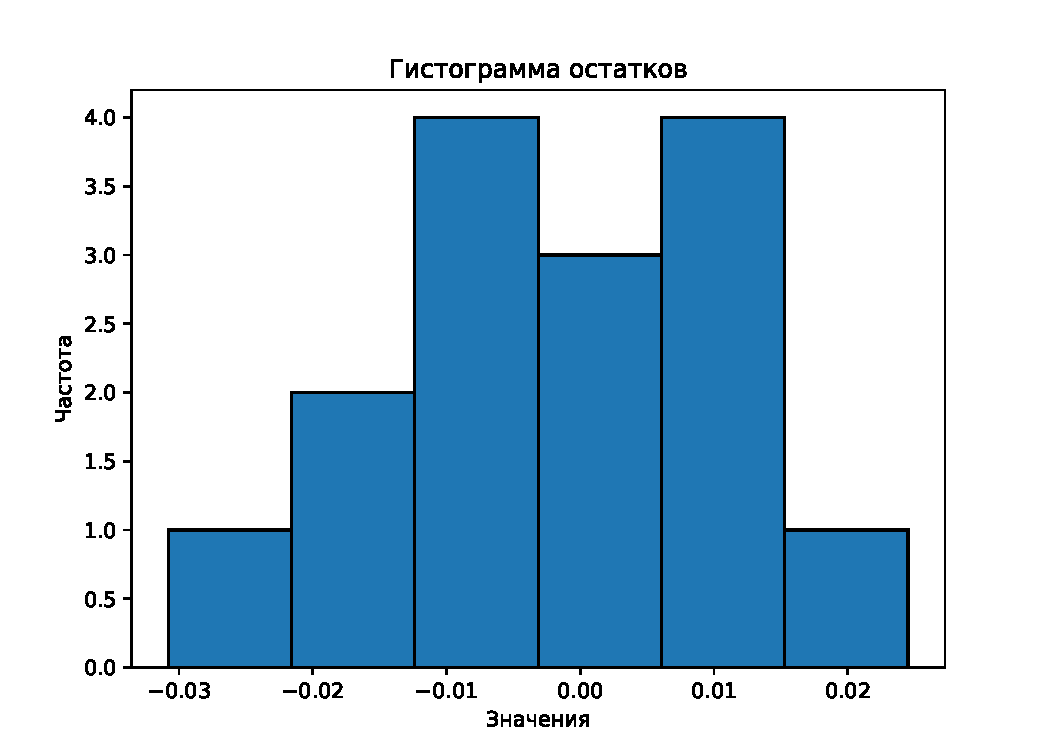
\includegraphics[width=0.7\linewidth]{gist.pdf}
    \caption{Гистограмма распределения остатков}    
\end{figure}
Распределение остатков сильно похоже на нормальное. Проверим это точно, воспользовавшись методом Шапиро Уилка:
\begin{equation}
	W = \frac{(\sum_{i=1}^{n}\omega_i \cdot x_i)^2}{\sum_{i=1}^{n}(x_i - <x>)^2}
\end{equation}
где $x_i$ - упорядоченные по возрастанию значения в выборке, $\omega_i$ -  весовые коэффициенты, которые зависят от ожидаемых значений упорядоченной нормально распределенной выборки,
 $<x>$ - среднее значение выборки. \par
 Пусть $H_0$ - гипотеза, что остатки распределены нормально \par
 Посчитаем значение статистики $W$:
 \begin{equation}
	W = 0.95 \;\;\;\;\;\;\;\; p_{\text{значение}} = 0,47
 \end{equation}
 Тогда при 5\% уровне значимости можем утверждать в соответствие с тестом Шапиро-Уилка, что данные распределены нормально(не отвергаем $H_0$ )

 Проверим данные на гомоскедатичность. Воспользуемся тестом Уайта. Определим статистику:
 \begin{equation}
	\text{White's statistic} = n \cdot R^2 = 3,27 \;\;\;\;\;\;\;\; p_{\text{значение}} = 0,2
 \end{equation}
 Получаем что для 5\% уровня значимости $p_{\text{значение}} > 0,05$, что позволяет нам не отклонить гипотезу $H_0$, и сделать вывод о гомоскедатичности остатков.

 Итак, теперь, убедившись в выполнении необходимых условий, можем вычислить параметры регрессии методом Монте-Карло. Моделировать точки будем следующим образом:
 \begin{equation}
	x_i^{\text{новое}} = x_i + \mathcal{N}(0, \sigma_{x_i}) 
 \end{equation}
 \begin{equation}
	y_i^{\text{новое}} = y_i + \mathcal{N}(0, \sqrt{\sigma_{y_i}^2 + RMSE^2}) 
 \end{equation}
 Будем проводить $N = 1000$ итераций. Гистограмма распределения представлена на (рис.2). А сам результат:
 \begin{figure}[h!]
    \centering
    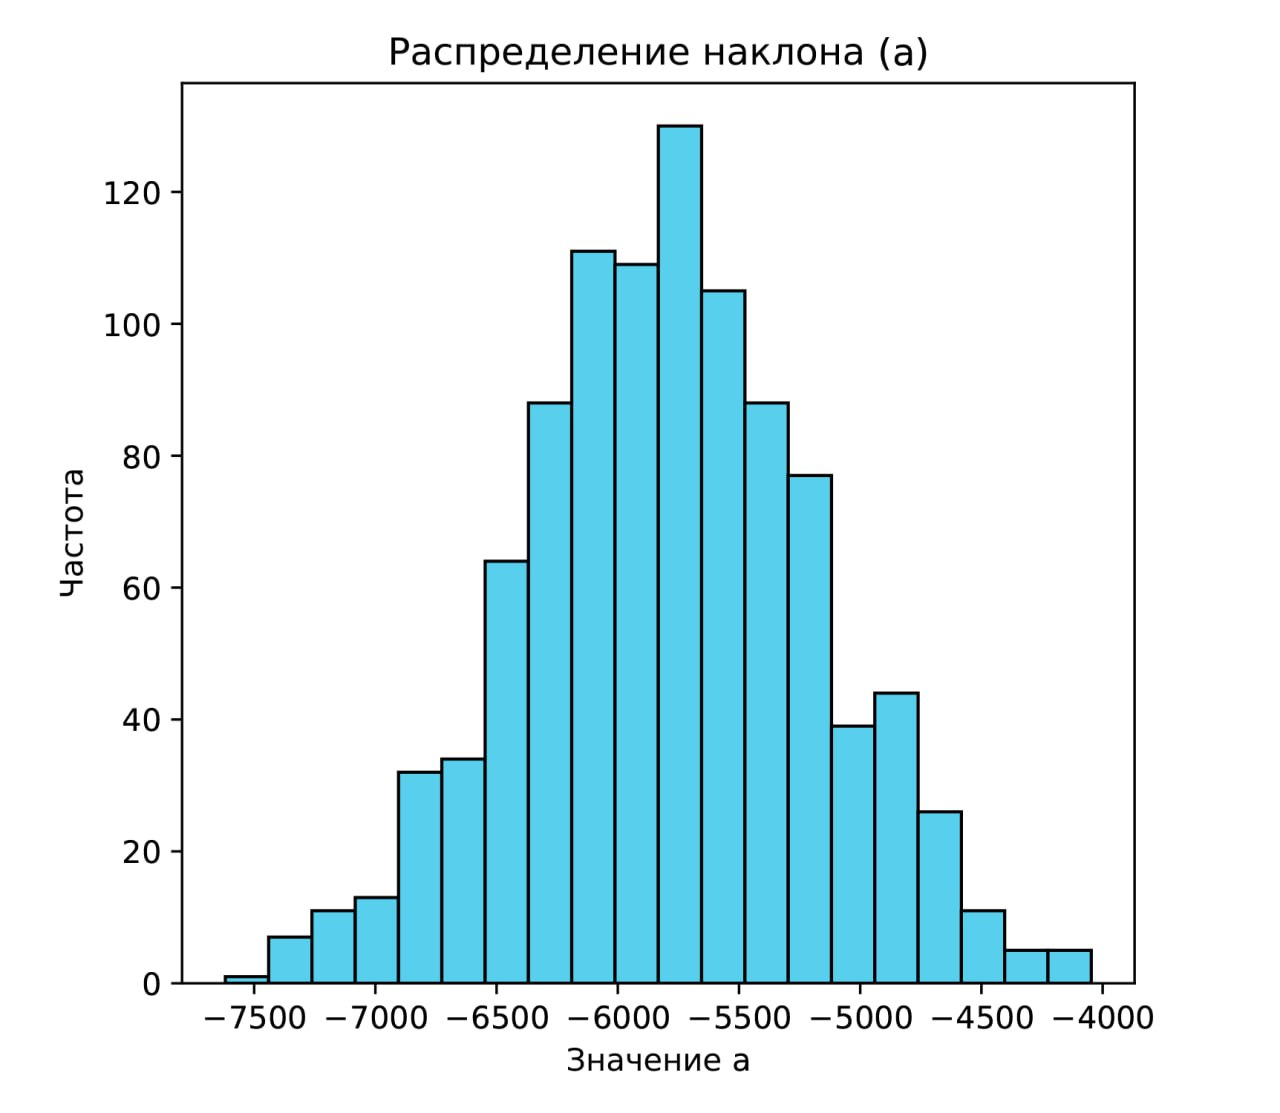
\includegraphics[width=0.6\linewidth]{gist_first.jpg}
    \caption{Гистограмма коэфициента наклона в методе Монте-Карло}    
\end{figure}
 \begin{equation}
	a = -5779.29 ± 616.83 \;\;\;\;\;\;\; L = 48,02 \pm 5,12
 \end{equation}
 В итоге, получается, что в данном методе, мы исправили все минусы предшествующих методов.
 \subsection{Метод Бутсрэпа}
Данный метод заключается в том, что на основе данных создаётся бустрэп-выборка, то есть из данных многократно генерируются новые подвыборки с повторением, и 
по каждой подвыборке строится линейная модель. После этого среднее все коэфициентов наклона усредняется, а в качесвте погрешности берется стандратное отклонение. \par
В нашем случае получаются следующие параметры:
\begin{equation}
	a_{mean}= -5756 \;\;\;\;\;\;\;\; a_{std} = 475
 \end{equation}
 А итоговое значение
 \begin{equation}
	L= 47,83 \pm 3,95
 \end{equation}

 Таким образом, полученное значение оказалось чуть менее точным чем в методе Монте-Карло, однако
 нам не потребовалось делать дополнительных действий по оценке распределения остатков.

\subsection{Результаты}
Как мы видим, применение более продвинутых статистических методов не позволило значительно улучшить значение исследуемой величины, так как прирост в точности составил около 5\%.
Тем не менее, мы получили намного более точную погрешность, которая позволила в пределах 1,5 - 2 $\sigma$ согласовать табличное значение с экспериментальным. 
Таким образом, мы видим, что применение более точных методов, позволило изменить вывод о согласии теории с экспериментом.
Также рассмотрим, насколько такая большая погрешность справедлива. Построим регрессионную прямую (рис.3):
\begin{figure}[h!]
    \centering
    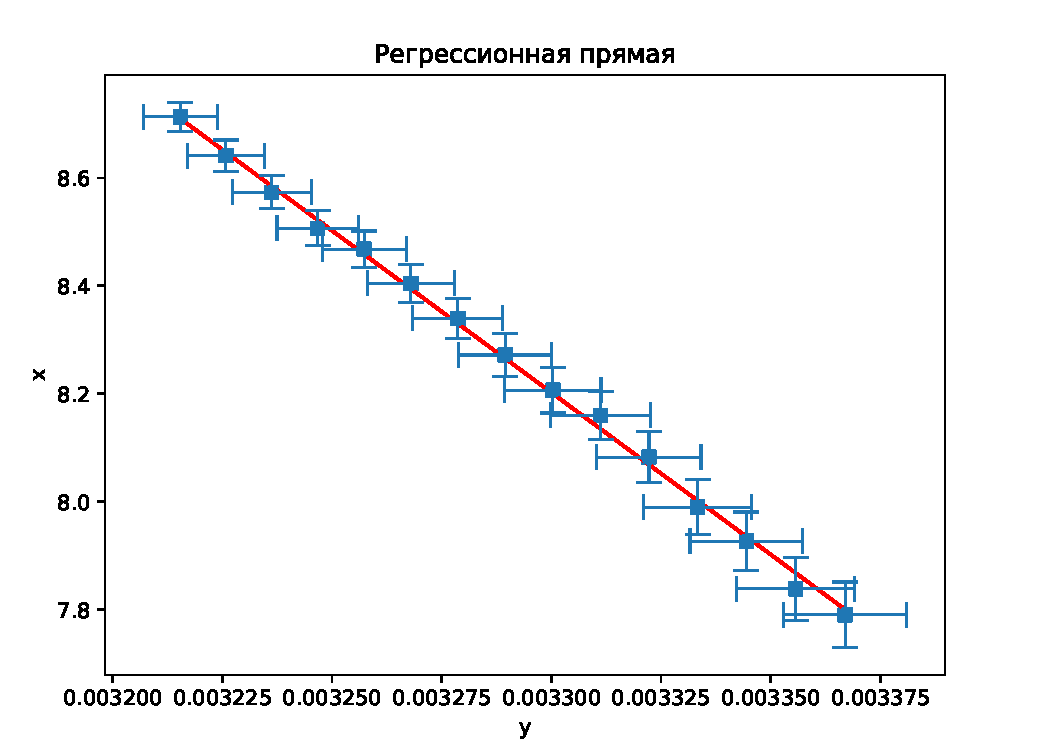
\includegraphics[width=0.7\linewidth]{linear_regression.pdf}
    \caption{График линейной регрессии.}    
\end{figure}
Оценим, в какие предельные прямые можно провести через планки погрешностей (рис. 4)
\begin{figure}[h!]
    \centering
    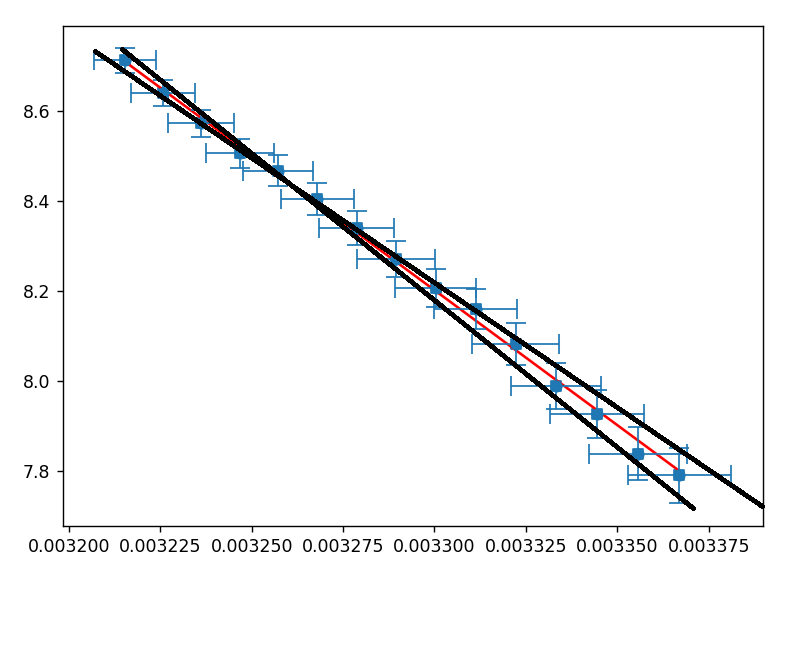
\includegraphics[width=0.7\linewidth]{differnet line.png}
    \caption{Предельные прямые}    
\end{figure}
Значения прямых лежат лежат в диапазоне:
\begin{equation}
	-63000 < k < - 5300
\end{equation}
Это даём нам основания предполагать, что погрешность коэфициента наклона в самом деле может принимать те значения, которые мы получили в ходе обработки.

\newpage
\section{Влияние статистического метода на значение искомой величины}
Рассмотрим как применение тех или иных способов для вычисления регрессионных параметров может повлиять на результаты исследования
\subsection{Экспермиентальные данные}
В качестве экспериментальных данных возьмем резульатты измерения постоянной времени $\tau$ интегрирующей цепочки в лабораторной работе 3.6.1
\begin{table}[H]
	\centering
	\begin{tabular}{|c|c|}
		\hline
		K& $\nu$, кГц \\ \hline
		0,164 & 300      \\ \hline
		0,094 & 600      \\ \hline
		0,055 & 900      \\ \hline
		0,039 & 1200      \\ \hline
		0,035 & 1500      \\ \hline
		0,027 & 1800      \\ \hline
		0,024 & 2100      \\ \hline
		0,015 & 2400      \\ \hline
	\end{tabular}
	\caption{Данные из лабораторной работы 2.4.1}
	\label{tab:izm}

\end{table}
В данном разделе будет в большей степени показано влияние различных методов на само значение исследуемой величины, а также показано, как некорректное применение методов
при невыполнении тех или иных условий может дать неправильный результат.
\subsection{Метод МНК}
Воспользуемся формулой для расчёта наклона наилучшей прямой:
\begin{equation}
	a = \frac{<xy> - <x><y>}{<x^2>-<x>^2} \;\;\;\;\;\;\; \sigma_a = \sqrt{\frac{1}{n-1}(\frac{D_{yy}}{D_{xx}} - a^2)} 
\end{equation}
Посчитаем численно значение коэфициента наклона
\begin{equation}
	a = 3,13 \cdot10^{-6} \;\;\;\;\;\;\; \sigma_a = 0,12\cdot10^{-6}
\end{equation}
Так как полученная погрешность отображает случайную погрешность, уточним её, добавив систематическую погрешность
\begin{equation}
	\sigma_{\text{сист}} = a \cdot \varepsilon_{K}
\end{equation}
Тогда итоговая погрешность, которая учитывает как случайную так и систематичскую погрешности:
\begin{equation}
	\sigma_{total} = \sqrt{\sigma_{\text{случ}}^2 + \sigma_{\text{сист}}^2} = 0,44\cdot10^{-6} 
\end{equation}
Тогда если мы посчитаем теплоту парообразования:
\begin{equation}
	\tau_{\text{exp}} = (3,13 \pm 0,44 )\cdot10^{-6} \text{     c} \;\;\;\;\;\;\;\; \tau_{\text{табл}} = 3\cdot10^{-6}  \text{     c}
\end{equation}
Как видим, значение совпадает в пределах погрешности, однако само значение отличается от истинного на $\approx 5\%$. Попробуем это исправить.
\subsection{Одномерный метод $\chi^2$}
Так как мы исследуем данные на линейную зависиомость $y = a + bx$, то определим функцию $\chi^2$ следующим видом:
\begin{equation}
	\chi^2(a, b) = \sum_{i=1}^{n} \frac{(y_i-(a+bx_i))^2}{\sigma^2_{y_i}}
\end{equation}
Будем минимизировать эту функцию, тем самым получим параметр $\chi^2$ наилучшей прямой. Тогда получим:
\begin{equation}
	a = 3,07\cdot10^{-6} 
\end{equation}
Найдем погрешность коэфициента, найдя взвешенные остатки:
\begin{equation}
	\sigma_{\text{остатки}}^2 = \frac{1}{n-2} \sum_{i=1}^{n}\frac{(y_i-(a+bx_i))^2}{\sigma^2_{y_i}} \;\;\;\;\;\;\;\; \sigma_b = \sigma_{\text{остатки}}\cdot \sqrt{\frac{1}{\sum \frac{(x_i-<x>)^2}{\sigma_{y_i}^2}}}
\end{equation}
Получим:
\begin{equation}
	\sigma_b = 0,17 \cdot10^{-6} \;\;\;\;\;\;\;\;\;\;\; \sigma_{total} = \sqrt{\sigma_{\text{случ}}^2 + \sigma_{\text{сист}}^2} = 0,46
\end{equation}
Тогда если мы посчитаем временную постоянную
\begin{equation}
	\tau_{\text{exp}} = (3,07 \pm 0,46 )\cdot10^{-6} \text{     c} \;\;\;\;\;\;\;\; 
\end{equation}
Отметим несколько особенностей использованного метода:
\begin{itemize}
	\item По сравнению с прошлым метоодом(МНК), погрешность сильно не изменилось
	\item Однако, на целых 3\% изменилось само исследуемое значение. Это говорит о более высокой точности оценки параметра 
\end{itemize}
Результат апроксимации приведён на (рис. 5)
\begin{figure}[h!]
    \centering
    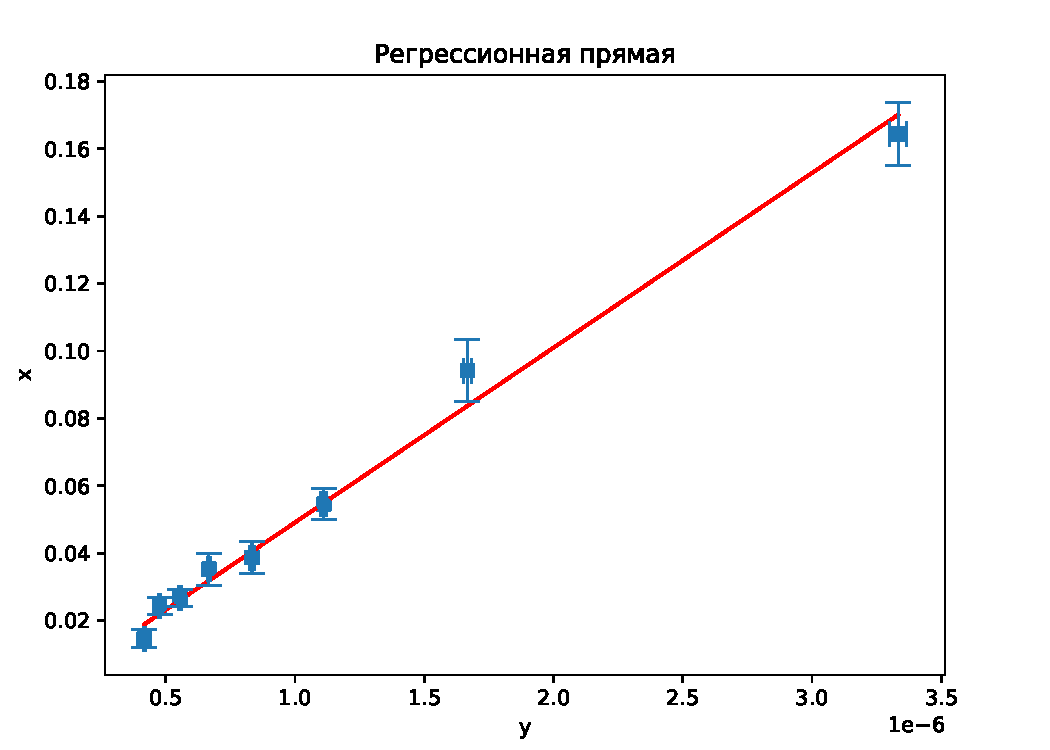
\includegraphics[width=0.7\linewidth]{tau_graph.pdf}
    \caption{Линейная апроксимация}    
\end{figure}
\subsection{Расчёт коэфициента наклона методом двумерной взвешенной регрессии}
Определим функцию $\chi^2$ в случае двумерной взвешенной регрессии
\begin{equation}
	\chi^2(a, b) = \sum_{i=1}^{n} \frac{(y_i-(a+bx_i))^2}{\sigma^2_{y_i}+ b^2\sigma_{x_i}^2}
\end{equation}
Для того, чтобы получить коэфициент $b$, воспользуемся одним из предыдущих методом, чтобы оценить параметр, после этого проведем повторную подгонку.
\begin{equation}
	a = - 3,07 \;\;\;\;\;\;\;\;\; 
\end{equation}
Вычислим погрешности для коэфициента наклона:
\begin{equation}
	\sigma_{\text{остатки}}^2 = \sqrt{\frac{\chi^2}{n-2}} \;\;\;\;\;\;\;\;\; \sigma_a = \sigma_{\text{остатки}}\cdot \sqrt{\frac{1}{\sum \frac{(x_i-<x>)^2}{\sigma^2_{y_i}+ b^2\sigma_{x_i}^2}}}
\end{equation}
Получим в итоге значения:
\begin{equation}
	\tau_{\text{exp}} = (3,07 \pm 0,46 )\cdot10^{-6}  \text{     c} \;\;\;\;\;\;\;\; 
\end{equation}
Как видим, с точностью до второго знака, значения совпали с предыдущим пунктом. Поймем причины этого
\begin{itemize}
	\item Данный пример нагялдно показывает, что применение метода $\chi^2$ порой черевато огромными неточностями. Мы отчётливо видим,
что в случае, когда погрешность по оси абсцисс была ощутимой, наши значение в предыдущем разделе изменили оцень внушительно. Сейчас же, когда мы можем пренебречь погрешностями
по оси абсцисс, отличие между одномерной и двумерной регрессией практически отсутствуют(как минимум с точностью до второго знака после запятой)
Это показывает, что что хоть метод $\chi^2$ и даёт большую точность по сравнению с привычным МНК, но использование его "упрощенной" версии, не всегда можеть быть корректно, а порой 
может привести и к большим неточностям при обработке результатов.
\end{itemize}
\subsection{Метод Монте-Карло}
Попробуем применить метод Монте-Карло в данном случае. 
Аналогично, чтобы можно было применить его корректно, должны выполянться два условия. \par
1) Остатки должны быть распределены нормально\par
2) Гомоскедатичность остатков \par
Для того чтобы оценить распределение остатков, построим гистограмму (рис.1)
\begin{figure}[h!]
    \centering
    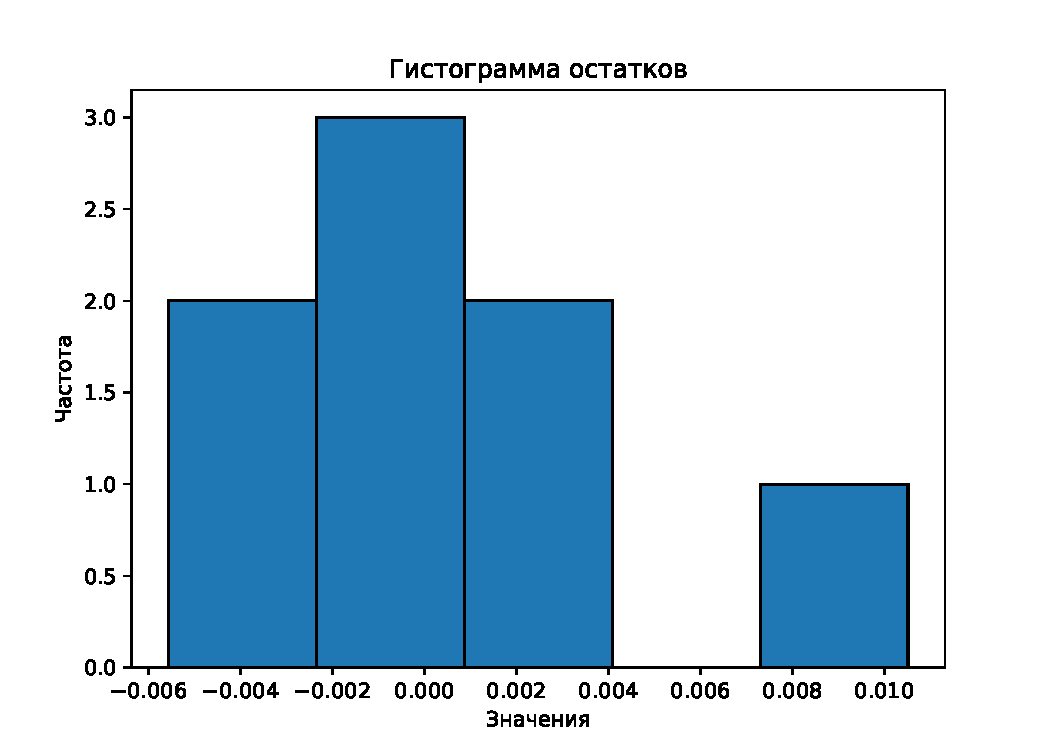
\includegraphics[width=0.7\linewidth]{gist_uncorrect.pdf}
    \caption{Гистограмма распределения остатков}    
\end{figure}
Как и в предыдущем разделе, распределение очень похоже на нормальное. Однако, давайте проведем тест Шапиро-Уилка.
\begin{equation}
	W = \frac{(\sum_{i=1}^{n}\omega_i \cdot x_i)^2}{\sum_{i=1}^{n}(x_i - <x>)^2}
\end{equation}
где $x_i$ - упорядоченные по возрастанию значения в выборке, $\omega_i$ -  весовые коэффициенты, которые зависят от ожидаемых значений упорядоченной нормально распределенной выборки,
 $<x>$ - среднее значение выборки. \par
 Пусть $H_0$ - гипотеза, что остатки распределены нормально \par
 Посчитаем значение статистики $W$:
 \begin{equation}
	W = 0.81 \;\;\;\;\;\;\;\; p_{\text{значение}} = 0,04
 \end{equation}
 Однако в отличие от предыдущего случая, при 5\% уровне значимости НЕЛЬЗЯ утверждать, что данные распределены нормально(отвергаем $H_0$ )

 Проверим данные на гомоскедатичность. Воспользуемся тестом Уайта. Определим статистику:
 \begin{equation}
	\text{White's statistic} = n \cdot R^2 = 3,72 \;\;\;\;\;\;\;\; p_{\text{значение}} = 0,16
 \end{equation}
 Получаем что для 5\% уровня значимости $p_{\text{значение}} > 0,05$, что позволяет нам не отклонить гипотезу $H_0$, и сделать вывод о гомоскедатичности остатков.

Так как одно из условий невыполняется, то применять корректно метод Монте-Карло нельзя. Посмотрим, что в самом деле результаты не совсем будут соответствовать нашим ожиданиям.

 \begin{equation}
	x_i^{\text{новое}} = x_i + \mathcal{N}(0, \sigma_{x_i}) 
 \end{equation}
 \begin{equation}
	y_i^{\text{новое}} = y_i + \mathcal{N}(0, \sqrt{\sigma_{y_i}^2 + RMSE^2}) 
 \end{equation}
 \begin{figure}[h!]
    \centering
    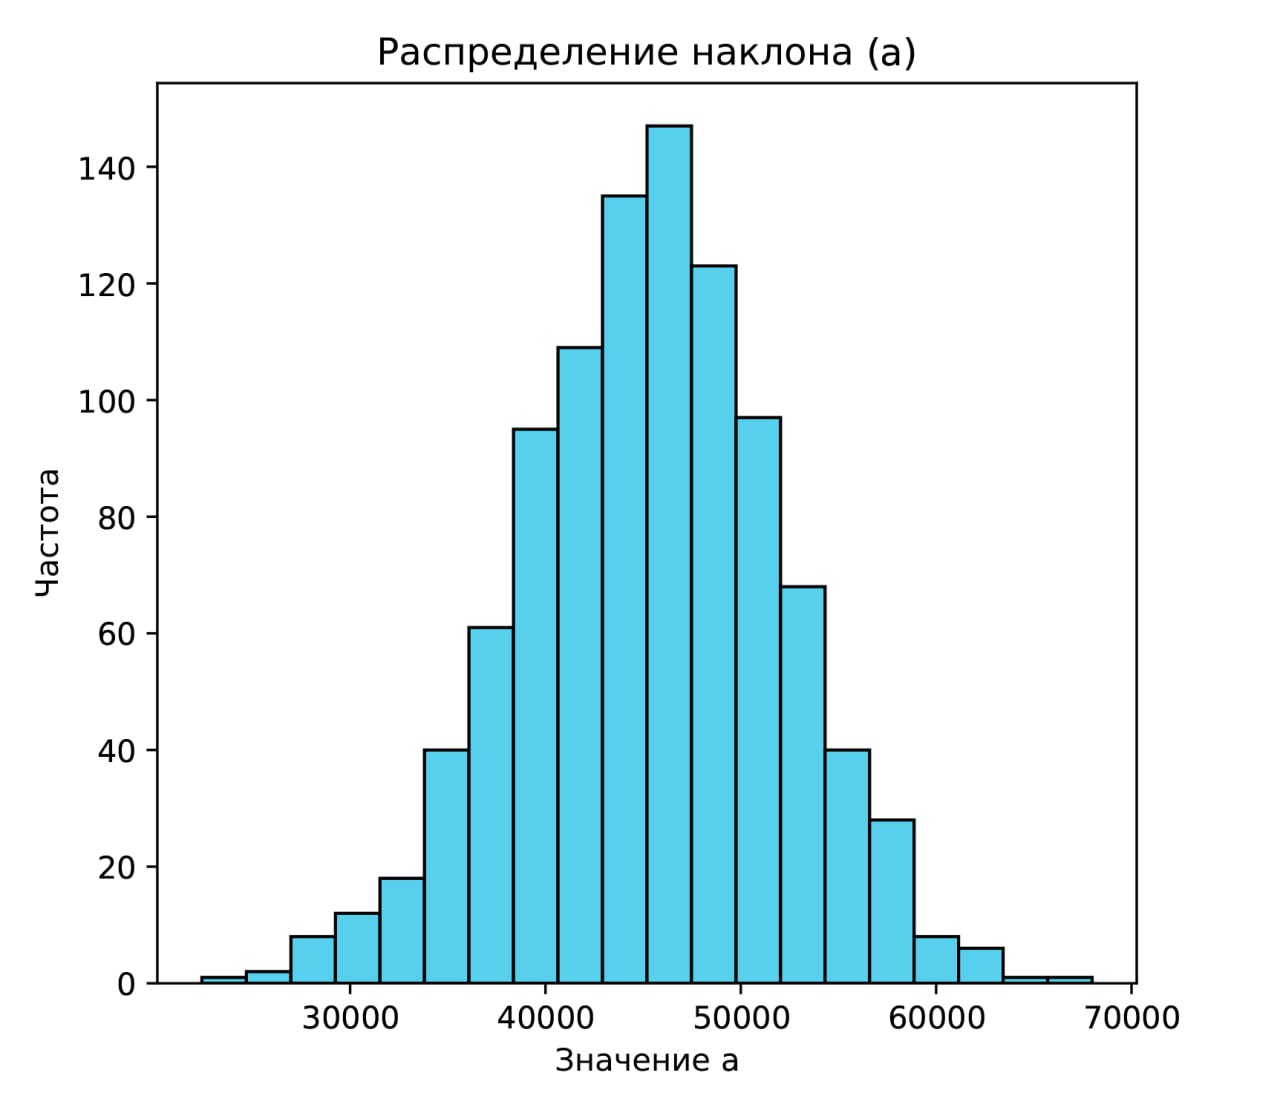
\includegraphics[width=0.7\linewidth]{gist_second.jpg}
    \caption{Гистограмма наклона в методе Монте-Карло}    
\end{figure}
\begin{equation}
	\tau_{\text{exp}} = (3,5 \pm 0,5 )\cdot10^{-6} \text{     c} \;\;\;\;\;\;\;\; 
\end{equation}
Как мы видим, значение в сравнение с прошлыми результатами очень сильно отклонилось от ожидаемого, хотя метод Монте-Карло должен работать точнее, чем предыдущие.
Этот пример, показывает важность соблюдения учёта необходимых условий при применении того или иного метода.

\newpage
\section{Влияние на статстического метода на малые погешности}
Бывают случаи, когда величина погрешностей по каждой из осей мала по отноешнию к величие, и может сложиться впечатление,
что и погрешность регрессионной прямой также будет пренебрижима мала. Однако, не всегда это может быть правдой, и применение более сложных статистических методов может выявить наличие более значимой ошибки коэфициентов.
\subsection{Экспериментальные данные}
Возьмём в качестве примера такой набор данных:

\begin{table}[H]
	\centering
	\begin{tabular}{|c|c|c|c|}
		\hline
		x& y & $\sigma_{x}$  & $\sigma_{y}$  \\ \hline
		1 & 3,9  & 0,00001  & 0,05           \\ \hline
		2 & 7,9  & 0,00001  & 0,05           \\ \hline
		3 & 11,9  & 0,00001  & 0,05           \\ \hline
		4 & 15,9  & 0,00001  & 0,05           \\ \hline
		5 & 19,9  & 0,00001  & 0,05           \\ \hline
		6 & 23,9  & 0,00001  & 0,05           \\ \hline
		7 & 27,9  & 0,00001  & 0,05           \\ \hline

	\end{tabular}
	\caption{Данные из лабораторной работы 2.4.1}
	\label{tab:izm}

\end{table}

\subsection{Сравнение статистических методов}
Посчитаем коэфициент наклона для приведённого набора данных различными методами. Все результаты занесем в таблицу

\begin{table}[H]
	\centering
	\begin{tabular}{|c|c|c|c|}
		\hline
		Статистический метод& a & $\sigma_{a}$ \\ \hline
		МНК & 4,0  & 4,2 $\cdot 10^{-8}$          \\ \hline
		Одномерный $\chi^2$ & 3,9999  & 0,0067           \\ \hline
		Двумерный $\chi^2$  & 3,9999  & 0,0094            \\ \hline
		Метод Монте-Карло & 3,9999  & 0,0014         \\ \hline
		Бутстрэп & 3,9999  &  0,0095           \\ \hline
		
	\end{tabular}
	\caption{Данные из лабораторной работы 2.4.1}
	\label{tab:izm}

\end{table}

Как можно заметить, использование простого метода наименьших квадратов не даёт представление об истинной погрешности, поскольку 
значением порядка $10^{-8}$ можно принебречь. Исходя из этих данных можно было бы сделать неверный вывод о высокой точности измерений. 
Однако, применяя остальные статистические методы, можно заметить, что относительная неточность соствляет порядка $0,25 \%$, что также не является большой величиной,
но она показывает что ошибки в измерениях присутствуют и они вносят погрешность в итоговые измерения.



\section{Результаты}
В ходе проделанной работы, мы рассмотрели как применение разлчных статистических методом позволяет улучшить интерпретацию данных полученных при физическом эксперименте.
На примере трёх наборов данных, мы получили сначала более корректный учёт ошибок, во втором более корректный учёт значений, а в третьем показали, что важно использовать более сложные статистические методы, чтобы получать корректное представление о погрешностях.
Сравнили методы между собой, показали их основные достоинства и недостатки. На реальном примере убедились в важности соблюдения тех или иных условий при применении определённых
методов.

\end{document}
